\documentclass[]{article}
\usepackage{lmodern}
\usepackage{amssymb,amsmath}
\usepackage{ifxetex,ifluatex}
\usepackage{fixltx2e} % provides \textsubscript
\ifnum 0\ifxetex 1\fi\ifluatex 1\fi=0 % if pdftex
  \usepackage[T1]{fontenc}
  \usepackage[utf8]{inputenc}
\else % if luatex or xelatex
  \ifxetex
    \usepackage{mathspec}
  \else
    \usepackage{fontspec}
  \fi
  \defaultfontfeatures{Ligatures=TeX,Scale=MatchLowercase}
\fi
% use upquote if available, for straight quotes in verbatim environments
\IfFileExists{upquote.sty}{\usepackage{upquote}}{}
% use microtype if available
\IfFileExists{microtype.sty}{%
\usepackage{microtype}
\UseMicrotypeSet[protrusion]{basicmath} % disable protrusion for tt fonts
}{}
\usepackage[margin=1in]{geometry}
\usepackage{hyperref}
\hypersetup{unicode=true,
            pdftitle={Returrners\_dataset},
            pdfauthor={Z.CAI},
            pdfborder={0 0 0},
            breaklinks=true}
\urlstyle{same}  % don't use monospace font for urls
\usepackage{color}
\usepackage{fancyvrb}
\newcommand{\VerbBar}{|}
\newcommand{\VERB}{\Verb[commandchars=\\\{\}]}
\DefineVerbatimEnvironment{Highlighting}{Verbatim}{commandchars=\\\{\}}
% Add ',fontsize=\small' for more characters per line
\usepackage{framed}
\definecolor{shadecolor}{RGB}{248,248,248}
\newenvironment{Shaded}{\begin{snugshade}}{\end{snugshade}}
\newcommand{\AlertTok}[1]{\textcolor[rgb]{0.94,0.16,0.16}{#1}}
\newcommand{\AnnotationTok}[1]{\textcolor[rgb]{0.56,0.35,0.01}{\textbf{\textit{#1}}}}
\newcommand{\AttributeTok}[1]{\textcolor[rgb]{0.77,0.63,0.00}{#1}}
\newcommand{\BaseNTok}[1]{\textcolor[rgb]{0.00,0.00,0.81}{#1}}
\newcommand{\BuiltInTok}[1]{#1}
\newcommand{\CharTok}[1]{\textcolor[rgb]{0.31,0.60,0.02}{#1}}
\newcommand{\CommentTok}[1]{\textcolor[rgb]{0.56,0.35,0.01}{\textit{#1}}}
\newcommand{\CommentVarTok}[1]{\textcolor[rgb]{0.56,0.35,0.01}{\textbf{\textit{#1}}}}
\newcommand{\ConstantTok}[1]{\textcolor[rgb]{0.00,0.00,0.00}{#1}}
\newcommand{\ControlFlowTok}[1]{\textcolor[rgb]{0.13,0.29,0.53}{\textbf{#1}}}
\newcommand{\DataTypeTok}[1]{\textcolor[rgb]{0.13,0.29,0.53}{#1}}
\newcommand{\DecValTok}[1]{\textcolor[rgb]{0.00,0.00,0.81}{#1}}
\newcommand{\DocumentationTok}[1]{\textcolor[rgb]{0.56,0.35,0.01}{\textbf{\textit{#1}}}}
\newcommand{\ErrorTok}[1]{\textcolor[rgb]{0.64,0.00,0.00}{\textbf{#1}}}
\newcommand{\ExtensionTok}[1]{#1}
\newcommand{\FloatTok}[1]{\textcolor[rgb]{0.00,0.00,0.81}{#1}}
\newcommand{\FunctionTok}[1]{\textcolor[rgb]{0.00,0.00,0.00}{#1}}
\newcommand{\ImportTok}[1]{#1}
\newcommand{\InformationTok}[1]{\textcolor[rgb]{0.56,0.35,0.01}{\textbf{\textit{#1}}}}
\newcommand{\KeywordTok}[1]{\textcolor[rgb]{0.13,0.29,0.53}{\textbf{#1}}}
\newcommand{\NormalTok}[1]{#1}
\newcommand{\OperatorTok}[1]{\textcolor[rgb]{0.81,0.36,0.00}{\textbf{#1}}}
\newcommand{\OtherTok}[1]{\textcolor[rgb]{0.56,0.35,0.01}{#1}}
\newcommand{\PreprocessorTok}[1]{\textcolor[rgb]{0.56,0.35,0.01}{\textit{#1}}}
\newcommand{\RegionMarkerTok}[1]{#1}
\newcommand{\SpecialCharTok}[1]{\textcolor[rgb]{0.00,0.00,0.00}{#1}}
\newcommand{\SpecialStringTok}[1]{\textcolor[rgb]{0.31,0.60,0.02}{#1}}
\newcommand{\StringTok}[1]{\textcolor[rgb]{0.31,0.60,0.02}{#1}}
\newcommand{\VariableTok}[1]{\textcolor[rgb]{0.00,0.00,0.00}{#1}}
\newcommand{\VerbatimStringTok}[1]{\textcolor[rgb]{0.31,0.60,0.02}{#1}}
\newcommand{\WarningTok}[1]{\textcolor[rgb]{0.56,0.35,0.01}{\textbf{\textit{#1}}}}
\usepackage{graphicx,grffile}
\makeatletter
\def\maxwidth{\ifdim\Gin@nat@width>\linewidth\linewidth\else\Gin@nat@width\fi}
\def\maxheight{\ifdim\Gin@nat@height>\textheight\textheight\else\Gin@nat@height\fi}
\makeatother
% Scale images if necessary, so that they will not overflow the page
% margins by default, and it is still possible to overwrite the defaults
% using explicit options in \includegraphics[width, height, ...]{}
\setkeys{Gin}{width=\maxwidth,height=\maxheight,keepaspectratio}
\IfFileExists{parskip.sty}{%
\usepackage{parskip}
}{% else
\setlength{\parindent}{0pt}
\setlength{\parskip}{6pt plus 2pt minus 1pt}
}
\setlength{\emergencystretch}{3em}  % prevent overfull lines
\providecommand{\tightlist}{%
  \setlength{\itemsep}{0pt}\setlength{\parskip}{0pt}}
\setcounter{secnumdepth}{0}
% Redefines (sub)paragraphs to behave more like sections
\ifx\paragraph\undefined\else
\let\oldparagraph\paragraph
\renewcommand{\paragraph}[1]{\oldparagraph{#1}\mbox{}}
\fi
\ifx\subparagraph\undefined\else
\let\oldsubparagraph\subparagraph
\renewcommand{\subparagraph}[1]{\oldsubparagraph{#1}\mbox{}}
\fi

%%% Use protect on footnotes to avoid problems with footnotes in titles
\let\rmarkdownfootnote\footnote%
\def\footnote{\protect\rmarkdownfootnote}

%%% Change title format to be more compact
\usepackage{titling}

% Create subtitle command for use in maketitle
\providecommand{\subtitle}[1]{
  \posttitle{
    \begin{center}\large#1\end{center}
    }
}

\setlength{\droptitle}{-2em}

  \title{Returrners\_dataset}
    \pretitle{\vspace{\droptitle}\centering\huge}
  \posttitle{\par}
    \author{Z.CAI}
    \preauthor{\centering\large\emph}
  \postauthor{\par}
      \predate{\centering\large\emph}
  \postdate{\par}
    \date{2021年11月24日}


\begin{document}
\maketitle

\hypertarget{the-returners-dataset}{%
\section{The Returners DataSet}\label{the-returners-dataset}}

loading the returners dataset

\begin{Shaded}
\begin{Highlighting}[]
\FunctionTok{library}\NormalTok{(keras)}

\NormalTok{reuters }\OtherTok{\textless{}{-}} \FunctionTok{dataset\_reuters}\NormalTok{(}\AttributeTok{num\_words =} \DecValTok{10000}\NormalTok{)}
\end{Highlighting}
\end{Shaded}

\begin{verbatim}
## Warning in normalizePath(path.expand(path), winslash, mustWork):
## path[1]="C:\Users\CAI\anaconda3\envs\rstudio_conda/python.exe": 系统找不到
## 指定的文件。
\end{verbatim}

\begin{verbatim}
## Warning in normalizePath(path.expand(path), winslash, mustWork):
## path[1]="C:\Users\CAI\anaconda3\envs\tensorflow_2.6/python.exe": 系统找不到
## 指定的文件。
\end{verbatim}

\begin{verbatim}
## Warning in normalizePath(path.expand(path), winslash, mustWork):
## path[1]="C:\Users\CAI\anaconda3\envs\rstudio_conda/python.exe": 系统找不到
## 指定的文件。
\end{verbatim}

\begin{verbatim}
## Warning in normalizePath(path.expand(path), winslash, mustWork):
## path[1]="C:\Users\CAI\anaconda3\envs\tensorflow_2.6/python.exe": 系统找不到
## 指定的文件。
\end{verbatim}

\begin{verbatim}
## Loaded Tensorflow version 2.6.1
\end{verbatim}

\begin{Shaded}
\begin{Highlighting}[]
\FunctionTok{c}\NormalTok{(}\FunctionTok{c}\NormalTok{(train\_data, train\_labels), }\FunctionTok{c}\NormalTok{(test\_data, test\_labels)) }\SpecialCharTok{\%\textless{}{-}\%}\NormalTok{ reuters}
\end{Highlighting}
\end{Shaded}

\begin{Shaded}
\begin{Highlighting}[]
\FunctionTok{length}\NormalTok{(train\_data)}
\end{Highlighting}
\end{Shaded}

\begin{verbatim}
## [1] 8982
\end{verbatim}

\begin{Shaded}
\begin{Highlighting}[]
\FunctionTok{length}\NormalTok{(test\_data)}
\end{Highlighting}
\end{Shaded}

\begin{verbatim}
## [1] 2246
\end{verbatim}

\begin{Shaded}
\begin{Highlighting}[]
\NormalTok{train\_data[[}\DecValTok{1}\NormalTok{]]}
\end{Highlighting}
\end{Shaded}

\begin{verbatim}
##  [1]    1    2    2    8   43   10  447    5   25  207  270    5 3095  111
## [15]   16  369  186   90   67    7   89    5   19  102    6   19  124   15
## [29]   90   67   84   22  482   26    7   48    4   49    8  864   39  209
## [43]  154    6  151    6   83   11   15   22  155   11   15    7   48    9
## [57] 4579 1005  504    6  258    6  272   11   15   22  134   44   11   15
## [71]   16    8  197 1245   90   67   52   29  209   30   32  132    6  109
## [85]   15   17   12
\end{verbatim}

decoding newswires back to text

\begin{Shaded}
\begin{Highlighting}[]
\NormalTok{word\_index }\OtherTok{\textless{}{-}} \FunctionTok{dataset\_reuters\_word\_index}\NormalTok{()}
\NormalTok{reverse\_word\_index }\OtherTok{\textless{}{-}} \FunctionTok{names}\NormalTok{(word\_index) }
\FunctionTok{names}\NormalTok{(reverse\_word\_index) }\OtherTok{\textless{}{-}}\NormalTok{ word\_index}
\NormalTok{decoded\_newswire }\OtherTok{\textless{}{-}} \FunctionTok{sapply}\NormalTok{(train\_data[[}\DecValTok{1}\NormalTok{]], }\ControlFlowTok{function}\NormalTok{(index) \{}
\NormalTok{  word }\OtherTok{\textless{}{-}} \ControlFlowTok{if}\NormalTok{ (index }\SpecialCharTok{\textgreater{}=} \DecValTok{3}\NormalTok{) reverse\_word\_index[[}\FunctionTok{as.character}\NormalTok{(index }\SpecialCharTok{{-}} \DecValTok{3}\NormalTok{)]]}
  \ControlFlowTok{if}\NormalTok{ (}\SpecialCharTok{!}\FunctionTok{is.null}\NormalTok{(word)) word }\ControlFlowTok{else} \StringTok{"?"} 
\NormalTok{  \})}

\NormalTok{decoded\_newswire}
\end{Highlighting}
\end{Shaded}

\begin{verbatim}
##  [1] "?"           "?"           "?"           "said"        "as"         
##  [6] "a"           "result"      "of"          "its"         "december"   
## [11] "acquisition" "of"          "space"       "co"          "it"         
## [16] "expects"     "earnings"    "per"         "share"       "in"         
## [21] "1987"        "of"          "1"           "15"          "to"         
## [26] "1"           "30"          "dlrs"        "per"         "share"      
## [31] "up"          "from"        "70"          "cts"         "in"         
## [36] "1986"        "the"         "company"     "said"        "pretax"     
## [41] "net"         "should"      "rise"        "to"          "nine"       
## [46] "to"          "10"          "mln"         "dlrs"        "from"       
## [51] "six"         "mln"         "dlrs"        "in"          "1986"       
## [56] "and"         "rental"      "operation"   "revenues"    "to"         
## [61] "19"          "to"          "22"          "mln"         "dlrs"       
## [66] "from"        "12"          "5"           "mln"         "dlrs"       
## [71] "it"          "said"        "cash"        "flow"        "per"        
## [76] "share"       "this"        "year"        "should"      "be"         
## [81] "2"           "50"          "to"          "three"       "dlrs"       
## [86] "reuter"      "3"
\end{verbatim}

\begin{Shaded}
\begin{Highlighting}[]
\NormalTok{train\_labels[[}\DecValTok{1}\NormalTok{]]}
\end{Highlighting}
\end{Shaded}

\begin{verbatim}
## [1] 3
\end{verbatim}

encoding the data

\begin{Shaded}
\begin{Highlighting}[]
\NormalTok{vectorize\_sequences }\OtherTok{\textless{}{-}} \ControlFlowTok{function}\NormalTok{(sequences, }\AttributeTok{dimension =} \DecValTok{10000}\NormalTok{) \{ }
\NormalTok{  results }\OtherTok{\textless{}{-}} \FunctionTok{matrix}\NormalTok{(}\DecValTok{0}\NormalTok{, }\AttributeTok{nrow =} \FunctionTok{length}\NormalTok{(sequences), }\AttributeTok{ncol =}\NormalTok{ dimension) }
  \ControlFlowTok{for}\NormalTok{ (i }\ControlFlowTok{in} \DecValTok{1}\SpecialCharTok{:}\FunctionTok{length}\NormalTok{(sequences))}
\NormalTok{    results[i, sequences[[i]]] }\OtherTok{\textless{}{-}} \DecValTok{1} 
\NormalTok{  results}
\NormalTok{\}}

\NormalTok{x\_train }\OtherTok{\textless{}{-}} \FunctionTok{vectorize\_sequences}\NormalTok{(train\_data) }
\NormalTok{x\_test }\OtherTok{\textless{}{-}} \FunctionTok{vectorize\_sequences}\NormalTok{(test\_data)}

\FunctionTok{str}\NormalTok{(x\_train)}
\end{Highlighting}
\end{Shaded}

\begin{verbatim}
##  num [1:8982, 1:10000] 1 1 1 1 1 1 1 1 1 1 ...
\end{verbatim}

\begin{Shaded}
\begin{Highlighting}[]
\FunctionTok{str}\NormalTok{(x\_test)}
\end{Highlighting}
\end{Shaded}

\begin{verbatim}
##  num [1:2246, 1:10000] 1 1 1 1 1 1 1 1 1 1 ...
\end{verbatim}

\begin{Shaded}
\begin{Highlighting}[]
\NormalTok{to\_one\_hot }\OtherTok{\textless{}{-}} \ControlFlowTok{function}\NormalTok{(labels, }\AttributeTok{dimension =} \DecValTok{46}\NormalTok{) \{}
\NormalTok{  results }\OtherTok{\textless{}{-}} \FunctionTok{matrix}\NormalTok{(}\DecValTok{0}\NormalTok{, }\AttributeTok{nrow =} \FunctionTok{length}\NormalTok{(labels), }\AttributeTok{ncol =}\NormalTok{ dimension) }
  \ControlFlowTok{for}\NormalTok{ (i }\ControlFlowTok{in} \DecValTok{1}\SpecialCharTok{:}\FunctionTok{length}\NormalTok{(labels))}
\NormalTok{    results[i, labels[[i]] }\SpecialCharTok{+} \DecValTok{1}\NormalTok{] }\OtherTok{\textless{}{-}} \DecValTok{1}
\NormalTok{  results}
\NormalTok{\}}

\NormalTok{one\_hot\_train\_labels }\OtherTok{\textless{}{-}} \FunctionTok{to\_one\_hot}\NormalTok{(train\_labels)}
\NormalTok{one\_hot\_test\_labels }\OtherTok{\textless{}{-}} \FunctionTok{to\_one\_hot}\NormalTok{(test\_labels)}

\FunctionTok{str}\NormalTok{(one\_hot\_train\_labels)}
\end{Highlighting}
\end{Shaded}

\begin{verbatim}
##  num [1:8982, 1:46] 0 0 0 0 0 0 0 0 0 0 ...
\end{verbatim}

\begin{Shaded}
\begin{Highlighting}[]
\FunctionTok{str}\NormalTok{(one\_hot\_test\_labels)}
\end{Highlighting}
\end{Shaded}

\begin{verbatim}
##  num [1:2246, 1:46] 0 0 0 0 0 0 0 0 0 0 ...
\end{verbatim}

model definition

\begin{Shaded}
\begin{Highlighting}[]
\NormalTok{model }\OtherTok{\textless{}{-}} \FunctionTok{keras\_model\_sequential}\NormalTok{() }\SpecialCharTok{\%\textgreater{}\%}
  \FunctionTok{layer\_dense}\NormalTok{(}\AttributeTok{units =} \DecValTok{64}\NormalTok{, }\AttributeTok{activation =} \StringTok{"relu"}\NormalTok{, }\AttributeTok{input\_shape =} \FunctionTok{c}\NormalTok{(}\DecValTok{10000}\NormalTok{)) }\SpecialCharTok{\%\textgreater{}\%} 
  \FunctionTok{layer\_dense}\NormalTok{(}\AttributeTok{units =} \DecValTok{64}\NormalTok{, }\AttributeTok{activation =} \StringTok{"relu"}\NormalTok{) }\SpecialCharTok{\%\textgreater{}\%}
  \FunctionTok{layer\_dense}\NormalTok{(}\AttributeTok{units =} \DecValTok{46}\NormalTok{, }\AttributeTok{activation =} \StringTok{"softmax"}\NormalTok{)}
\end{Highlighting}
\end{Shaded}

compiling the model

\begin{Shaded}
\begin{Highlighting}[]
\NormalTok{model }\SpecialCharTok{\%\textgreater{}\%} \FunctionTok{compile}\NormalTok{(}
  \AttributeTok{optimizer =} \StringTok{"rmsprop"}\NormalTok{,}
  \AttributeTok{loss =} \StringTok{"categorical\_crossentropy"}\NormalTok{, }
  \AttributeTok{metrics =} \FunctionTok{c}\NormalTok{(}\StringTok{"accuracy"}\NormalTok{)}
\NormalTok{)}
\end{Highlighting}
\end{Shaded}

setting aside a validation set

\begin{Shaded}
\begin{Highlighting}[]
\NormalTok{val\_indices }\OtherTok{\textless{}{-}} \DecValTok{1}\SpecialCharTok{:}\DecValTok{1000}

\NormalTok{x\_val }\OtherTok{\textless{}{-}}\NormalTok{ x\_train[val\_indices,] }
\NormalTok{partial\_x\_train }\OtherTok{\textless{}{-}}\NormalTok{ x\_train[}\SpecialCharTok{{-}}\NormalTok{val\_indices,]}

\NormalTok{y\_val }\OtherTok{\textless{}{-}}\NormalTok{ one\_hot\_train\_labels[val\_indices,] }
\NormalTok{partial\_y\_train }\OtherTok{=}\NormalTok{ one\_hot\_train\_labels[}\SpecialCharTok{{-}}\NormalTok{val\_indices,]}
\end{Highlighting}
\end{Shaded}

training the model

\begin{Shaded}
\begin{Highlighting}[]
\NormalTok{history }\OtherTok{\textless{}{-}}\NormalTok{ model }\SpecialCharTok{\%\textgreater{}\%} \FunctionTok{fit}\NormalTok{(}
\NormalTok{  partial\_x\_train, }
\NormalTok{  partial\_y\_train,}
  \AttributeTok{epochs =} \DecValTok{20}\NormalTok{,}
  \AttributeTok{batch\_size =} \DecValTok{512}\NormalTok{,}
  \AttributeTok{validation\_data =} \FunctionTok{list}\NormalTok{(x\_val, y\_val)}
\NormalTok{)}
\end{Highlighting}
\end{Shaded}

plotting the training and validation metrics

\begin{Shaded}
\begin{Highlighting}[]
\FunctionTok{plot}\NormalTok{(history)}
\end{Highlighting}
\end{Shaded}

\begin{verbatim}
## `geom_smooth()` using formula 'y ~ x'
\end{verbatim}

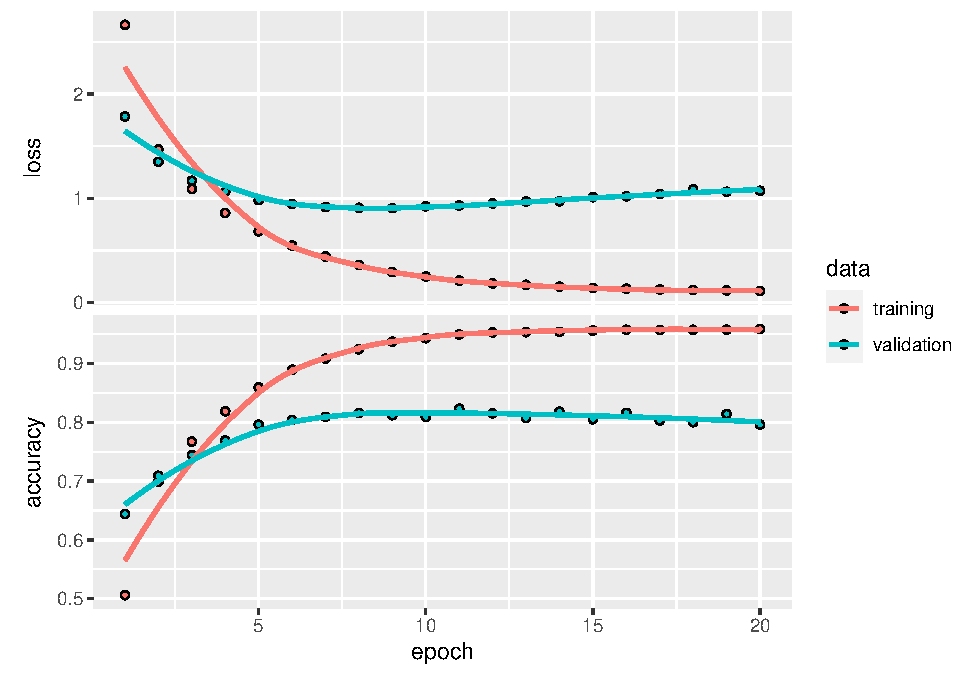
\includegraphics{Returners_dataset_files/figure-latex/unnamed-chunk-12-1.pdf}

retrainin a model from scratch

\begin{Shaded}
\begin{Highlighting}[]
\NormalTok{model }\OtherTok{\textless{}{-}} \FunctionTok{keras\_model\_sequential}\NormalTok{() }\SpecialCharTok{\%\textgreater{}\%}
  \FunctionTok{layer\_dense}\NormalTok{(}\AttributeTok{units =} \DecValTok{64}\NormalTok{, }\AttributeTok{activation =} \StringTok{"relu"}\NormalTok{, }\AttributeTok{input\_shape =} \FunctionTok{c}\NormalTok{(}\DecValTok{10000}\NormalTok{)) }\SpecialCharTok{\%\textgreater{}\%} 
  \FunctionTok{layer\_dense}\NormalTok{(}\AttributeTok{units =} \DecValTok{64}\NormalTok{, }\AttributeTok{activation =} \StringTok{"relu"}\NormalTok{) }\SpecialCharTok{\%\textgreater{}\%}
  \FunctionTok{layer\_dense}\NormalTok{(}\AttributeTok{units =} \DecValTok{46}\NormalTok{, }\AttributeTok{activation =} \StringTok{"softmax"}\NormalTok{)}

\NormalTok{model }\SpecialCharTok{\%\textgreater{}\%} \FunctionTok{compile}\NormalTok{(}
  \AttributeTok{optimizer =} \StringTok{"rmsprop"}\NormalTok{,}
  \AttributeTok{loss =} \StringTok{"categorical\_crossentropy"}\NormalTok{, }
  \AttributeTok{metrics =} \FunctionTok{c}\NormalTok{(}\StringTok{"accuracy"}\NormalTok{)}
\NormalTok{)}

\NormalTok{history }\OtherTok{\textless{}{-}}\NormalTok{ model }\SpecialCharTok{\%\textgreater{}\%} \FunctionTok{fit}\NormalTok{(}
\NormalTok{  partial\_x\_train, }
\NormalTok{  partial\_y\_train,}
  \AttributeTok{epochs =} \DecValTok{9}\NormalTok{,}
  \AttributeTok{batch\_size =} \DecValTok{512}\NormalTok{,}
  \AttributeTok{validation\_data =} \FunctionTok{list}\NormalTok{(x\_val, y\_val)}
\NormalTok{)}

\NormalTok{results }\OtherTok{\textless{}{-}}\NormalTok{ model }\SpecialCharTok{\%\textgreater{}\%} \FunctionTok{evaluate}\NormalTok{(x\_test, one\_hot\_test\_labels)}
\NormalTok{results}
\end{Highlighting}
\end{Shaded}

\begin{verbatim}
##      loss  accuracy 
## 0.9980597 0.7871772
\end{verbatim}

compare a random baseline

\begin{Shaded}
\begin{Highlighting}[]
\NormalTok{test\_labels\_copy }\OtherTok{\textless{}{-}}\NormalTok{ test\_labels}
\NormalTok{test\_labels\_copy }\OtherTok{\textless{}{-}} \FunctionTok{sample}\NormalTok{(test\_labels\_copy)}
\FunctionTok{length}\NormalTok{(}\FunctionTok{which}\NormalTok{(test\_labels }\SpecialCharTok{==}\NormalTok{ test\_labels\_copy)) }\SpecialCharTok{/} \FunctionTok{length}\NormalTok{(test\_labels)}
\end{Highlighting}
\end{Shaded}

\begin{verbatim}
## [1] 0.1959038
\end{verbatim}

generate predictions for new data

\begin{Shaded}
\begin{Highlighting}[]
\NormalTok{predictions }\OtherTok{\textless{}{-}}\NormalTok{ model }\SpecialCharTok{\%\textgreater{}\%} \FunctionTok{predict}\NormalTok{(x\_test)}

\FunctionTok{dim}\NormalTok{(predictions)}
\end{Highlighting}
\end{Shaded}

\begin{verbatim}
## [1] 2246   46
\end{verbatim}

\begin{Shaded}
\begin{Highlighting}[]
\FunctionTok{sum}\NormalTok{(predictions[}\DecValTok{1}\NormalTok{,])}
\end{Highlighting}
\end{Shaded}

\begin{verbatim}
## [1] 1
\end{verbatim}

\begin{Shaded}
\begin{Highlighting}[]
\FunctionTok{which.max}\NormalTok{(predictions[}\DecValTok{1}\NormalTok{,])}
\end{Highlighting}
\end{Shaded}

\begin{verbatim}
## [1] 4
\end{verbatim}


\end{document}
